\documentclass[12pt]{article}
 \usepackage[margin=1in]{geometry} 
\usepackage{amsmath,amsthm,amssymb,amsfonts}
\usepackage{graphicx}

 
\newcommand{\N}{\mathbb{N}}
\newcommand{\Z}{\mathbb{Z}}
 
\newenvironment{problem}[2][]{\begin{trivlist}
\item[\hskip \labelsep {\bfseries #1}\hskip \labelsep {\bfseries #2.}]}{\end{trivlist}}

 
\begin{document}
  
\title{Computational Physics Project 1: Pendulum}
\author{Ben Zager, Remy Wang}
\maketitle
 
\begin{problem}{1}
	\textbf{Phase space of nonlinear pendulum}

\begin{figure}[ht!]
  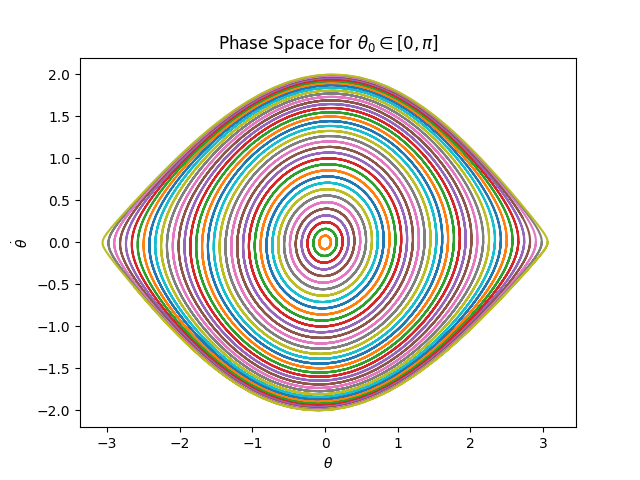
\includegraphics[scale=0.7]{../figures/phaseSpace.png}
  \caption{Plots of trajectory $(\theta,\dot{\theta})$, for many values of $\theta_{0} \in [0,\pi]$}
  \label{phase}
\end{figure}

\begin{figure}[ht!]
	\centering
	\begin{minipage}[b]{0.4\textwidth}
		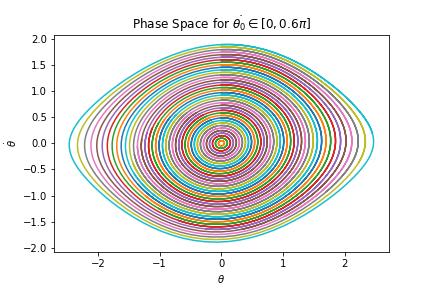
\includegraphics[scale=0.6]{../figures/phaseSpaceDot.png}
		\label{phaseDot}
	\end{minipage}
	\hfill
	\begin{minipage}[b]{0.4\textwidth}
		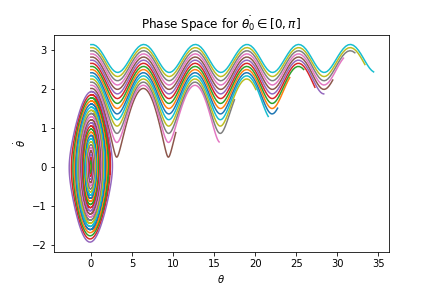
\includegraphics[scale=0.6]{../figures/phaseSpaceDot2.png}
		\label{phaseDot2}
	\end{minipage}
	\caption{Trajectory for various $\dot{\theta}$}
\end{figure}
\end{problem}
 
\begin{problem}{2}
	\textbf{Phase space of linear pendulum}
\begin{figure}[h!]
\centering
  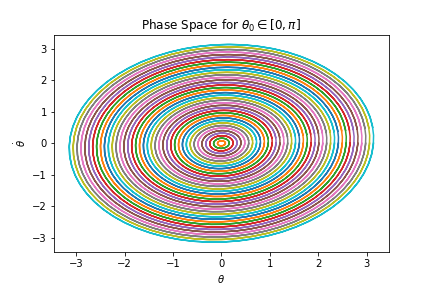
\includegraphics[scale=0.6]{../figures/phaseSpaceLinear.png}
  \caption{Plots of linearized trajectory $(\theta,\dot{\theta})$, for many values of $\theta_{0} \in [0,\pi]$}
  \label{phaseLin}
\end{figure}
\end{problem}

\begin{problem}{3}
	\textbf{Pendulum with driving force, $\gamma k^{2}cos(\omega t)$}
\end{problem}

\begin{problem}{4}
	\textbf{Exploration of driven system} \\
	For fixed $\theta$ and $\dot{\theta}$, how do the real and phase space trajectories vary with $\gamma$
\end{problem}

\begin{problem}{5}
	\textbf{Identifying $(\theta_{0},\gamma)$ for which the motion diverges}
\end{problem}

\begin{problem}{6}
	\textbf{Driven pendulum with damping} $\ddot{\theta}+2\beta\dot{\theta}+k^{2}sin\theta=\gamma k^{2}cos(\omega t)$ \\

\end{problem}

\begin{problem}{7}
	\textbf{Fourier analysis}
\end{problem}


\end{document}